\documentclass{article}

\usepackage{graphicx}
\usepackage{amsmath}
\usepackage{amsfonts}
\usepackage{algorithm2e}
\usepackage{float}
\usepackage{eso-pic}

\AddToShipoutPicture*{%
	\put(325, 660){
\includegraphics[height=1.7cm]{images/cpc.png}}
	\put(380, 670){
\includegraphics[height=1cm]{images/ieeecs.png}}
}

\begin{document}

\title{Learning Data Structures: Segment Trees}
\author{Lecturers Notes - CPC@UTEC}
\date{November 2020}

\maketitle

\setlength{\parskip}{7pt}
\setlength{\parindent}{0pt}

\section{Introduction}

Welcome to the CPC \& IEEE CS \textit{Learning Data Structures and algorithms} workshop! Today we will discuss a very important data structure in competitive programming: Segment trees.

\subsection{Problem}

Suppose we have and array $A$ of length $n$ with elements $A_1, A_2, A_3 \dots A_n$ and we need to find the same of elements in a range. More specifically, lets say we need to answer some queries of the form query$(l, r)$, such that:
$$\text{query}(l,r) = \sum_{i = l}^r A_i$$

\begin{itemize}
	\item Brute force solution in $O(n)$ per query.
	\item Fast $O(1)$ solution using \textit{prefix-sum}.
\end{itemize}

Now we want to support another type of operation: update$(i, x)$, adding $x$ to the element $A_i$. How can we do this?

\begin{itemize}
	\item Updating in $O(1)$ and querying in $O(n)$.
	\item Updating in $O(n)$ and querying in $O(1)$.
\end{itemize}

Both of this solutions have a worst case complexity of $O(qn)$. This is too slow! We need a better solution.

Now we can even complicate things more, what if we also needed to support another operation: update$(l, r, x)$, adding $x$ to all elements $A_i$ such that $l \leq i \leq r$.

All of this are very common scenarios when solving problems, so having a general and efficient solution for solving all of these would be a great addition to our problem-solving algorithmic toolbox.

\subsection{Divide \& Conquer}

\textit{Divide and conquer} is one of the most popular problem solving paradigms in computer science. The key idea is that we can solve a problem by dividing it into smaller similar problems. We can recursively do this until the solution is trivial, and then join the solutions of this \textit{sub-problems} in order to find the general solution. In general divide and conquer has 3 steps:

\begin{enumerate}
	\item \textbf{Divide:} Splitting the original problem in smaller sub-problems.
	\item \textbf{Conquer:} Solve each of this smaller problems (recursively).
	\item \textbf{Merge:} Joining the smaller solutions to find the global solution.
\end{enumerate}

\textbf{Examples:} Merge Sort, Sum

An interesting observation is that we can represent this problem / sub-problem structure as a tree, in which each node represents a problem and its children the sub-problems that need to be solved in order to find its solution:

\begin{figure}[H]
	\centering
	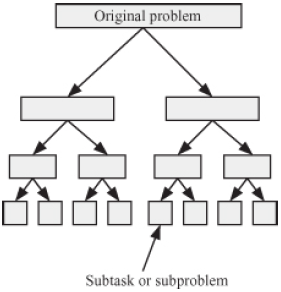
\includegraphics[width=0.5\linewidth]{images/divideandconquer}
\end{figure}

Now, what if we not only applied the divide and conquer algorithm, but also created this divide and conquer tree? 

\section{Segment Tree}

The solution to all the problems presented above is this \textit{divide and conquer tree} or as it is popularly known: \textit{segment tree}. This data structure will allow us to efficiently answer range updates and queries.

In general we can think of a segment tree as a \textit{binary tree} in which each node represents a range of values in an array, and each of the children represent a different half of this range:

\begin{figure}[H]
	\centering
	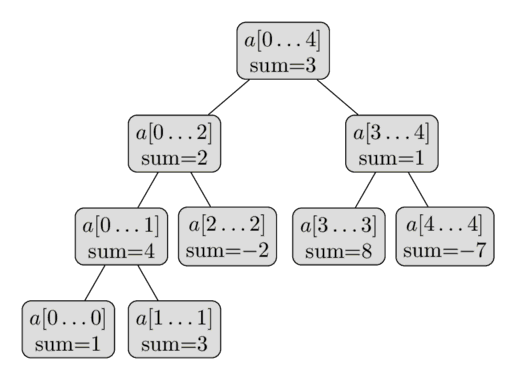
\includegraphics[width=0.5\linewidth]{images/segment-tree}
\end{figure}


In this lecture we will explore how we can use a segment tree to do the following operations efficiently:

\begin{itemize}
	\item \textbf{Point Update:} Updating a single value.
	\item \textbf{Range Query:} Solving a query for a range of values.
	\item \textbf{Range Update:} Updating a range of values.
\end{itemize}

The segment tree will allow us to realize all of this operations in $O(log(n))$ time with just $O(n)$ preprocessing. This will allow for an overall complexity of $O(n + qlgn)$, way better than the naive $O(qn)$ brute force complexity.

\subsection{Building a segment tree}

The first thing we need to do in order to use the \textit{segment tree} data structure, is to understand how we can transform a simple array into a segment tree. Lets say we have a node $v$ that represents the range $[l, r]$ of the original array, then it is clear that before finding the value of $st[v]$, we need to first find the value that will be stored in the two children of node $v$. 

As a segment tree is a binary tree we can use a smart indexing tree to easily maintain a tree structure, we will say that our tree is rooted at node $1$, and for every node $v$ its two children are nodes $2v$ and $2v + 1$.

We can combine these two ideas and arrive at the following algorithm:

\begin{algorithm}
	\SetAlgoNoLine
	\SetAlgoNoEnd
	\SetKwFunction{build}{build}
	\SetKwProg{void}{void}{}{}
	\void{\build{$v, l, r$}}{
		\If{$l = r$}{
			$st[v] \gets A[l]$\;
		}
		\Else {
			$m \gets \lfloor \frac{l + r}{2} \rfloor$\;
			\build{$2v, l, m$} \;
			\build{$2v + 1, m + 1, r$} \;
			$st[v] \gets st[2v] + st[2v + 1]$
		}
	}
\end{algorithm}

We can see that the time complexity of the construction of a segment tree obeys the following recurrence:

$T(n) = 2T\left(\frac{n}{2}\right) + O(1)$
$\implies T(n) = O(n)$

Therefore, in order to set up our segment tree we only need $O(n)$ preprocessing.

\subsection{Point Update}

Probably the easiest operation to understand is the point query operation. We can see the update operation as looking for the node that represents the $i$-th element of the array, updating it, and then updating the $O(log(n))$ nodes that contain that element according to the changes in the tree.

We can easily implement this algorithm using recursion:

\begin{algorithm}
	\SetAlgoNoLine
	\SetAlgoNoEnd
	\SetKwFunction{update}{update}
	\SetKwProg{void}{void}{}{}
	\void{\update{$v, l, r, i, x$}}{
		\If{$l = r$}{
			$st[v] \gets st[v] + x$\;
		}
		\Else {
			$m \gets \lfloor \frac{l + r}{2} \rfloor$\;
			\If{$i \leq m$}{
				\update{$2v, l, m, i, x$} \;
			}
			\Else{
				\update{$2v + 1, m + 1, r, i, x$} \;
			}
			$st[v] \gets st[2v] + st[2v + 1]$
		}
	}
\end{algorithm}

Evaluating the complexity of this solution is very simple. As in the general case at most one recursive call is made, we can express the complexity of the algorithm with the following recurrence:

$$T(n) = T\left(\frac{n}{2}\right) + O(1)$$
$$\implies T(n) = O(log(n))$$

\subsection{Range Query}

The range query operation, even though it can be intimidating at first, has a very similar idea to the point update operation at heart. Here instead of looking for the node that represents our index, we will need to look for the \textit{minimal set of nodes} that represent our range.

In order to better deal with these cases we will talk about three main situations:
\begin{itemize}
	\item Total coverage
	\item Partial coverage
	\item No coverage
\end{itemize}

The easy cases are the total and null coverage, as we can simply return the value stored in our node, or zero respectively. The tricky case is when there is partial coverage of our range: The node contains the points that we care about, but also have some additional points. In this case we can separate the problem in two sub-problems: looking for a solution in our left child and a solution in our right child. 

Using recursion and some implementation tricks to deal with edge cases, we can reach the following algorithm:

\begin{algorithm}[H]
	\SetAlgoNoLine
	\SetAlgoNoEnd
	\SetKwFunction{query}{query}
	\SetKwProg{int}{int}{}{}
	\int{\query{$v, l, r, ql, qr$}}{
		\If{$ql > qr$}{
			\Return $0$ \;
		}
		\If{$l = ql \land r = qr$}{
			\Return $st[v]$\;
		}
		$m \gets \lfloor \frac{l + r}{2} \rfloor$\;
		$vl \gets$ \query{$2v, l, m, ql, min(m, qr)$}\;
		$vr \gets$ \query{$2v + 1, m + 1, r, max(m  + 1, ql), qr$}\;
		\Return $vl + vr$\;
	}
\end{algorithm}

The time complexity of this algorithm is harder to analyze as with a naive glance it would appear that the recurrence this function obeys is:
$$T(n) = 2T\left(\frac{n}{2}\right) + O(1)$$
As there are two recursive calls. This would be bad, as it would imply that $T(n) = O(n)$. So why does this solution work?

The key observation is that in the general case, at least one of this recursive calls should be a base case, which would mean that in reality we only have one recursive call, giving us the same recurrence as point updates and therefore a complexity of $O(log(n))$.


\subsection{Range Update}

We already know how to range query, so range updating shouldn't be that different, right? Wrong. We could naively think that we can recycle our code for querying (with some minor changes), and have a working code for updating. At the end of the day we can efficiently edit the $O(logn)$ nodes that cover our range. For example, we could try something like the following algorithm:

\begin{algorithm}[H]
	\SetAlgoNoLine
	\SetAlgoNoEnd
	\SetKwFunction{update}{update}
	\SetKwProg{void}{void}{}{}
	\void{\update{$v, l, r, ql, qr$}}{
		\If{$ql > qr$}{
			\Return\;
		}
		\If{$l = ql \land r = qr$}{
			$st[v] \gets st[v] + x (r - l + 1)$\;
			\Return\;
		}
		$m \gets \lfloor \frac{l + r}{2} \rfloor$\;
		\update{$2v, l, m, ql, min(m, qr)$}\;
		\update{$2v + 1, m + 1, r, max(m  + 1, ql), qr$}\;
		$st[v] \gets st[2v] + st[2v + 1]$\;
	}
\end{algorithm}

However, there is a big problem with this solution: we are only updating the \textit{``topmost''} nodes that cover our range of interest, not all of them. What is worst is that we can show that our range is represented by $O(n)$ nodes, which means that in order to update all of them we should realize at least $O(n)$ operations. There must be a way of solving this problem

\subsection{Lazy Propagation}

The solution to the problem stated above is called \textit{lazy propagation}, and it allow us to update the $O(n)$ nodes that represent our range while keeping the $O(log(n))$ time per query.

Lazy propagation is a technique we can add to our data structures to amortize the complexity of some of the update operations in our data structure. Lazy propagation is \textbf{not a technique that can be exclusively used on segment trees}, \textit{Van Emde Boas trees}, \textit{tries}, and other tree-like structures.

The key idea of lazy propagation is that we can procrastinate updating some nodes until it is absolutely necessary. In practice this can be achieved by only updating some
of the nodes that cover our range of interest in the original update operation, and then amortizing the rest of updates in other operations such as queries and other updates. We will only update a set of nodes, and then \textit{lazily} propagate the changes when we need to access lower nodes.

\textbf{Example:} Lazy Propagation in Segment Tree

When properly used, lazy propagation should have a minor impact on our runtime complexity. In general, the complexity of all our operations will now be multiplied by a factor $T_{push}(n)$: the time complexity of our propagation. For this reason we need to ensure that our propagation is as efficient as possible.

\section{Segment Tree Variations}

Segment trees are a very broad topic for research and algorithmic development, thus they have many variations and techniques. Some of them that have gained popularity in the competitive programming sphere are:

\begin{itemize}
	\item Persistent segment tree
	\item Merge sort tree
	\item Segment tree beats
	\item Li-Chao tree
\end{itemize}

\begin{thebibliography}{9}
	\bibitem{cpalgorithms}
		CP-Algorithms: Segment Tree,\\
		\texttt{https://cp-algorithms.com/data\_structures/segment\_tree.html}

	\bibitem{DarthKnight}
		Algorithm Gym: Everything About Segment Trees,\\
		\texttt{https://codeforces.com/blog/entry/15890}

	\bibitem{AlgorithmsLive}
		Algorithms Live: Segment Tree,\\
		\texttt{https://youtu.be/Tr-xEGoByFQ}
	
	\bibitem{mit}
		MIT Open Coursware, Persistent Data Structures,\\
		\texttt{https://youtu.be/T0yzrZL1py0}
\end{thebibliography}

\end{document}
